Die Testüberdeckung wurde mithilfe von OpenCppCoverage auf Windows getestet.

\begin{figure}[H]
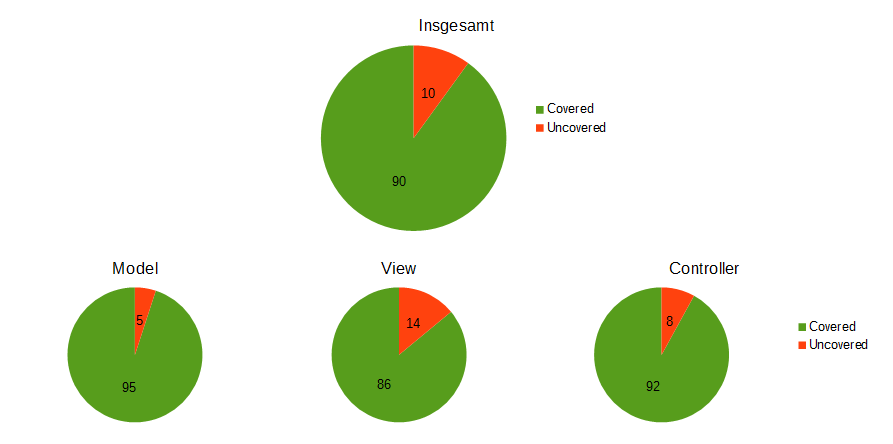
\includegraphics[width=1\linewidth]{img/Testszenarien}
\caption{Testüberdeckung der Testszenarien}
\label{fig:covCoBaB}
\end{figure}
Einerseits wurde die Überdeckung der zuvor beschriebenen, manuell durchgeführten Testszenarien und der Unit Tests bestimmt. Diese Überdeckung kann keine 100\% erreichen, da die Klassen zum Teil Methoden enthalten, die innerhalb von CoBaB nicht aufgerufen werden, sondern nur der Erweiterbarkeit oder besseren Benutzbarkeit für weitere Entwickler dienen. 

\begin{figure}[H]
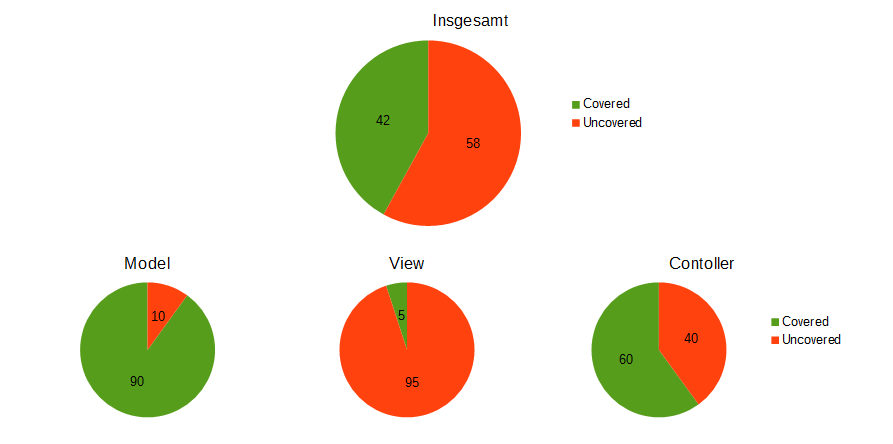
\includegraphics[width=1\linewidth]{img/UnitTests}
\caption{Testüberdeckung der Unit Tests}
\label{fig:covTests}
\end{figure}
Andererseits wurde die Überdeckung der 18 Klassen, die durch Unit Tests getestet wurden, gemessen. Diese Überdeckung ist nicht so hoch, da es für die View-Klassen keine Unit Tests gibt. 


Erzeugen der Ergebnisse:

CoBaB wurde mit OpenCppCoverage gestartet und TS10 ausgeführt:\smallskip\newline
OpenCppCoverage 
-\hspace{1pt}-sources \enquote{Pfad zu CoBaB\textbackslash CoBaB\textbackslash core} 
-\hspace{1pt}-sources \enquote{Pfad zu CoBaB\textbackslash CoBaB\textbackslash interface} 
-\hspace{1pt}-excluded\_sources *.h -\hspace{1pt}-export\_type=binary:CoBaB.cov 
-\hspace{1pt}- \newline \enquote{Pfad zu CoBaB\textbackslash CoBaB\textbackslash build-CoBaB-Desktop\_Qt\_5\_5\_1\_MSVC2013\_64bit-Debug  \textbackslash app\textbackslash debug\textbackslash CoBaB.exe}
\par

CoBaB wurde erneut mit OpenCppCoverage gestartet und TS30-TS90, TSW10-TSW60 und TSW80-TSW120 wurden ausgeführt, ohne CoBaB zu beenden: \smallskip\newline
OpenCppCoverage 
-\hspace{1pt}-sources \enquote{Pfad zu CoBaB\textbackslash CoBaB\textbackslash core} 
-\hspace{1pt}-sources \enquote{Pfad zu CoBaB\textbackslash CoBaB\textbackslash interface} 
-\hspace{1pt}-excluded\_sources *.h -\hspace{1pt}-export\_type=binary:CoBaB1.cov 
-\hspace{1pt}- \enquote{Pfad zu CoBaB\textbackslash CoBaB\textbackslash build-CoBaB-Desktop\_Qt\_5\_5\_1\_MSVC2013\_64bit-Debug \textbackslash app\textbackslash debug\textbackslash CoBaB.exe}
\par

CoBaB wurde mit Kommandozeilenargumenten und OpenCppCoverage gestartet, um TS20 und TSW70 gleichzeitig durchzuführen;\smallskip\newline
OpenCppCoverage 
-\hspace{1pt}-sources \enquote{Pfad zu CoBaB\textbackslash CoBaB\textbackslash core} 
-\hspace{1pt}-sources \enquote{Pfad zu CoBaB\textbackslash CoBaB\textbackslash interface} 
-\hspace{1pt}-excluded\_sources *.h -\hspace{1pt}-export\_type=binary:CoBaB2.cov 
-\hspace{1pt}- \enquote{Pfad zu CoBaB\textbackslash CoBaB\textbackslash build-CoBaB-Desktop\_Qt\_5\_5\_1\_MSVC2013\_64bit-Debug \textbackslash app\textbackslash debug\textbackslash CoBaB.exe} \enquote{Pfad zum Standardordner} -f
\par

Die Unit Tests zu CoBaB wurden ausgeführt und die Überdeckungsergebnisse zusammengefasst:\smallskip\newline
OpenCppCoverage 
-\hspace{1pt}-sources \enquote{Pfad zu CoBaB\textbackslash CoBaB\textbackslash core} 
-\hspace{1pt}-sources \enquote{Pfad zu CoBaB\textbackslash CoBaB\textbackslash interface} 
-\hspace{1pt}-excluded\_sources *.h -\hspace{1pt}-input\_coverage=CoBaB.cov -\hspace{1pt}-input\_ coverage=CoBaB1.cov -\hspace{1pt}-input\_coverage=CoBaB2.cov 
-\hspace{1pt}- \enquote{Pfad zu CoBaB\textbackslash CoBaB\textbackslash build-CoBaB-Desktop\_Qt\_5\_5\_1\_MSVC2013\_64bit-Debug\textbackslash test\textbackslash debug\textbackslash test.exe}
\newline
\par

Die Unit Tests wurden noch einmal alleine ausgeführt, um die Überdeckung nur durch die Unit Tests zu messen: \smallskip\newline
OpenCppCoverage 
-\hspace{1pt}-sources \enquote{Pfad zu CoBaB\textbackslash CoBaB\textbackslash core} 
-\hspace{1pt}-sources \enquote{Pfad zu CoBaB\textbackslash CoBaB\textbackslash interface} 
-\hspace{1pt}-excluded\_sources *.h 
-\hspace{1pt}-excluded\_modules *.dll
-\hspace{1pt}- \enquote{Pfad zu CoBaB\textbackslash CoBaB\textbackslash build-CoBaB-Desktop\_Qt\_5\_5\_1\_MSVC2013\_64bit-Debug \textbackslash test\textbackslash de-bug\textbackslash test.exe}
\par

Da die Ergebnisse von OpenCppCoverage nur die Klassen enthalten, die auch getestet wurden (also nicht die View Klassen), wurde die Überdeckung mithilfe der Ergebnisse der einzelnen Klassen manuell berechnet (überdeckte Zeilen/gesamte Zeilen). Insbesondere, um die Überdeckung von Model, View und Controller zu berechnen.